\documentclass[a4paper,11pt]{article}
\usepackage[utf8]{inputenc}
\usepackage[spanish]{babel}
\usepackage{fancyhdr}
\usepackage[pdftex]{graphicx}

\newenvironment{scaption}[1]{\caption{{\small #1}}}{}

\newenvironment{desig}{\begin{list}{}{\setlength{\labelsep}{0cm}\setlength{\labelwidth}{0cm}\setlength{\listparindent}{0cm}\setlength{\rightmargin}{\leftmargin}}}{\end{list}}


\author{Pablo Rodriguez Monetti}
\title{Introducción a la Arquitectura del Sistema Fastest}
\date{2008}

\begin{document}
 \maketitle
La arquitectura de un sistema de software define al sistema en términos de componentes y de conectores entre tales componentes. Los componentes son elementos tales como clientes y servidores, bases de datos, filtros, y capas en un sistema estratificado. Las interacciones entre componentes a este nivel de diseño pueden ser simples y familiares, tales como llamadas a procedimiento o acceso a variables compartidas. Pero pueden también ser complejas y semánticamente ricas, como lo son los protocolos cliente-servidor, protocolos de acceso a bases de datos, difusión de eventos y flujos de datos por tubos.

En particular, el sistema Fastest fue desarrollado sobre una arquitectura cliente/servidor. En este tipo de sistemas, un servidor representa un proceso que provee servicios a otros procesos (clientes). Es usual que el o los servidores no conozcan en principio la identidad de los clientes que tendrán acceso a ellos en tiempo de ejecución. Por otro lado, son los clientes quienes conocen la identidad de un servidor, o como es nuestro caso, pueden acceder a ella a través de otro servidor.
La principal motivación para la elección del mencionado estilo arquitectónico fue la de aprovechar de manera eficiente los recursos provistos por una red de computadoras.
Principalmente, lo que se persigue es obtener mayor performance ejecutando varias tareas en paralelo, pero además, poder correr más de un cliente del Fastest en distintas terminales. Todos los clientes deben consultar a un único repositorio de datos, ubicado en el llamado ''servidor de datos''. La cantidad de clientes y de servidores de cálculo del sistema no fue limitada.

Para que todos los componentes de una arquitectura cliente/servidor cooperen entre sí, se deben emplear ciertas técnicas de comunicación intercomponentes. En teoría, hay tres tipos básicos de técnicas de comunicación de procesamiento cooperativo que una arquitectura cliente/servidor puede usar:
\begin{itemize}
 \item{Tubos}
 \item{Llamadas a procedimiento remotas}
 \item{Interacciones cliente/servidor de SQL} 
\end{itemize}
Los tubos son mecanismos orientados a la conexión que pasan datos de un proceso a otro. En principio, los procesos pueden estar en diferentes máquinas, incluso corriendo sobre distintos sistemas operativos. Los detalles de los mecanismos de transporte soportados están ocultos a los usuarios de un tubo y los tubos imponen restricciones mímimas de protocolo y formato a los usuarios.

Una llamada a procedimiento remoto es un mecanismo por el cual un proceso puede ejecutar otro proceso (subrutina) que reside en un sistema diferente, y usualmente remoto, posiblemente corriendo en un sistema operativo diferente. Cualquier parámetro necesario para la subrutina es pasado entre el proceso original y el de la subrutina. Al igual que con los tubos, los detalles del mecanismo de transporte se ocultan al usuario de la llamada a procedimiento.

Una interacción cliente/servidor de SQL es un mecanismo que permite pasar consultas Structured Query Language (SQL) y los datos asociados a ellas de un proceso (usualmente un cliente) a otro proceso (servidor). Esta es un caso especial de interacción cliente/servidor, que se utiliza en el contexto de aplicaciones de base de datos relacionales distribuidas. En este caso, el servidor es el servidor de la base de datos relacional. Este puede residir en un sistema diferente y posiblemente corriendo en un sistema operativo distinto. Mientras los detalles de los mecanismos de transporte están ocultos por los desarrolladores de aplicaciones, las interacciones cliente/servidor de SQL imponen restricciones sveras de protocolos y formato a los usuarios.

En el caso del sistema Fastest, para realizar las interacciones entre clientes y servidores de cálculo se utilizaron unos tubos particulares llamados sockets. Para la comunicación entre clientes y servidores de cálculo con el servidor de datos se requirió el uso de interaciones cliente/servidor de SQL.

Hasta ahora solo hemos mencionado el uso del estilo arquitectónico cliente/servidor, como si nuestra arquitectura hubiera sido desarrollada en base a un estilo arquitectónico ''puro''. Sin embargo, y tal como sucede en la mayoría de los sistemas de considerable envergadura, es importante entender que Fastest involucra la combinación de más de un estilo arquitectónico: el cliente/servidor y la invocación implícita. Estos estilos se combinan jerárquicamente, dado que cada cliente de la arquitectura cliente/servidor es organizado de acuerdo a una arquitectura de invocación implícita.

La idea detrás de la invocación implícita es que en lugar de invocar un procedimiento directamente, un componente puede anunciar uno o más eventos. Otros componentes en el sistema pueden registrar interés en un evento asociándo a él un procedimiento. Cuando el evento es anunciado, el propio sistema (a través de un administrador de eventos) invoca a todos los procedimientos que anteriormente registraron interés en tal evento. Entonces, el anuncio de un evento ''implícitamente'' causa la invocación de procedimientos en otros módulos. En términos arquitectónicos, los componentes en un estilo de invocación implícita son módulos cuyas interfaces pueden proveer tanto una colección de procedimientos como un conjunto de eventos. Los procedimientos pueden ser invocados de la forma usual, pero un componente puede también registrar algunos de sus procedimientos con eventos del sistema. Esto causará que tales procedimientos sean invocados cuando los eventos de interés sean anunciados en tiempo de ejecución.


\begin{figure}
\begin{center}
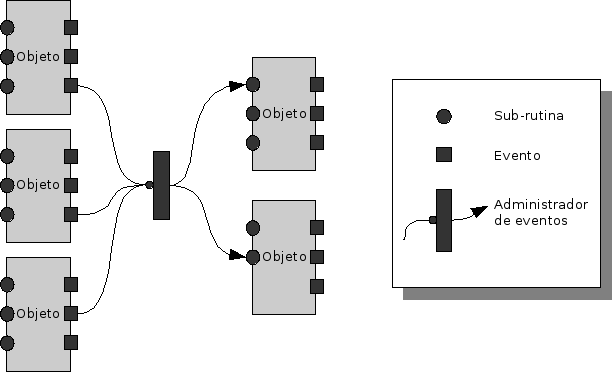
\includegraphics[scale=0.7]{/home/prodriguez/Fastest/Arquitectura/Introduccion/EstiloInvoc.png}
\end{center}
\end{figure}



El principal invariante del estilo es que los anunciantes de eventos no conocen qué componentes serán afectados por los eventos que pueden lanzar. Por esta razón, los componentes no tienen la posibilidad de hacer suposiciones acerca del orden de procesamiento, ni sobre si el procesamiento ocurrirá o no como resultado del anuncio de determinado evento. El beneficio más importante de este aspecto, y el principal motivo que nos llevó a elegir este estilo para organizar los clientes del sistema, es que facilita enormemente la evolución del sistema: los componentes pueden ser reemplazados por otros componentes o pueden agregarse otros nuevos sin afectar las interfaces de los ya existentes.

En nuestro sistema, esta capacidad dinámica de poder agregar y quitar componentes del sistema se controla a través de un archivo de configuración donde se indica qué procedimientos de qué componentes están interesados en qué eventos. Simplemente lo que se hace es leer este archivo de configuración al momento de iniciar el cliente del sistema, almacenando en una tabla dentro del administrador de eventos las relaciones entre eventos, componentes y procedimientos de componentes. Por esto, aunque la declaración de eventos es estática (dado que el conjunto posible de eventos queda fijado en tiempo de compilación), el binding entre eventos y procedimientos es dinámico: los componentes registran su interés en eventos en tiempo de ejecución. La declaración de eventos es centralizada: nos pareció suficiente contar con un único administrador de eventos. En cuanto a la estructura de los eventos, decidimos que los mismos tendrían una lista de parámetros por tipo de evento, es decir, cada evento tiene una lista fija de parámetros pero la cantidad y tipo puede ser diferente para cada evento.

Si bien en términos de arquitectura hablamos de invocación implícita, la implementación de este mecanismo se realizó a través de llamadas a procedimientos tradicionales. Esto es, el anuncio de un evento se lleva a cabo realizando la invocación explícita de una subrutina particular del administrador de eventos (módulo llamado EventAdmin), pasando como parámetro la instancia del módulo que representa al evento. El administrador simplemente consulta su tabla de eventos en busca de el o los procedimiento/s interesado/s en el evento, para luego realizar cada una de las invocaciones en un hilo de proceso diferente. Luego, es responsabilidad del componente ''invocado'' (esto es, del que se se invocó un procedimiento) obtener los parámetros relevantes del evento para llevar a cabo la tarea que le incumbe.

\begin{figure}
\begin{center}
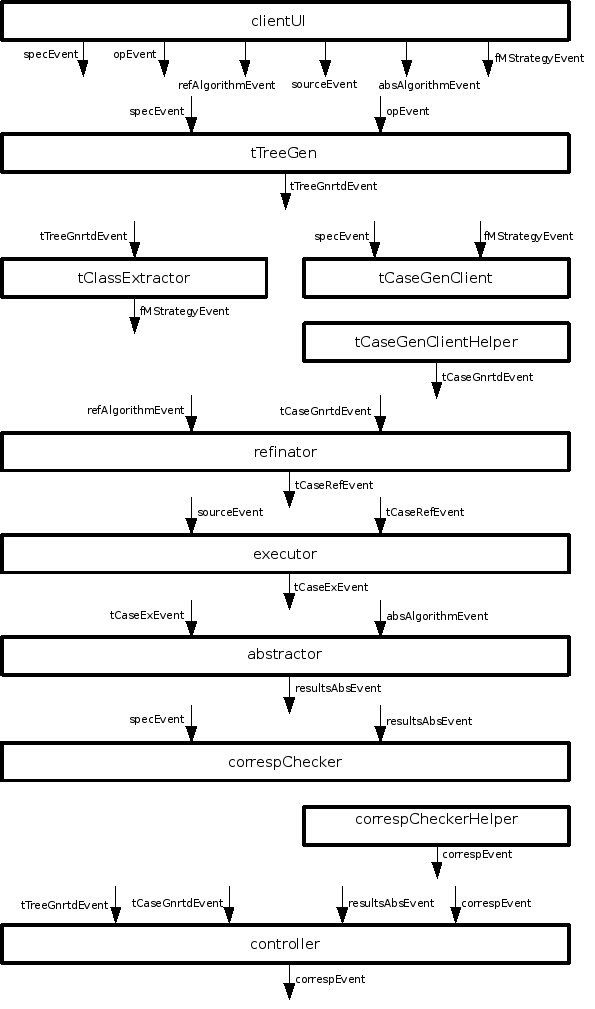
\includegraphics[scale=0.7]{/home/prodriguez/Fastest/Arquitectura/Introduccion/EsquemaGral.png}
\end{center}
\end{figure}

\end{document}

